%!TEX root = ..\Thesis.tex
\glsresetall

\chapter{Experimental validation of the step input estimation method }\label{chap:ExperimentalValidation}

\begin{quote}
\emph{The results of this chapter were published in Quintana Carapia, G., Markovsky, I. Pintelon, R., Csurcsia, P.Z., and Verbeke, D., "Experimental validation of a data-driven step input estimation method for dynamic measurements", IEEE Transactions on Instrumentation and Measurement Journal, 2019, doi: 10.1109/TIM.2019.2951865. \nocite{QuintanaTIM} }\vfill{}
\end{quote}

 \vfill{}

% \section{Introduction}

A measurement is a dynamic process. 
The sensor is a dynamic system that experiments changes after an input excitation.
The sensor output is first a transient state response and followed by a steady state response.

The influence of the input is observed in the sensor output, and thus it makes sense to estimate the input using the sensor response.
When the sensor reaches its steady-state, the input is a straightforwardly estimated from the sensor output making use of the sensor static gain.
To obtain a fast estimation, the sensor transient response must be considered instead of the steady state response.

A common approach is to filter the sensor transient response with another dynamic system to reduce the sensor transient time by inverting the sensor dynamics.
To design such a compensator system it is necessary a sensor model.
A different approach uses digital signal processing methods that are independent of the sensor model.
One of these methods is the data-driven method that estimates the unknown level of step inputs by processing the sensor step response. 
To assess the uncertainty of the data-driven step input estimation method, a experimental validation of this method was conducted in a real-life metrology application. 
This chapter describes the measurement experiments with a weighing sensor system and discuss the results observed.
The results are put in perspective to simulations and consider the measurement noise that is additive to the response of the sensor. 

The experimental results validate the data-driven step input estimation method, and indicate in which intervals of SNR and sample size the effectiveness of the method is guaranteed.


\begin{comment}
 In this paper we consider that a measurement is a dynamic process, where an input excites a dynamic system, the sensor, and causes a dynamic transient response that also depends on the initial conditions of the sensor.
The to-be-measured quantity is an unknown input that excites the sensor.
The consequent transient response is further processed to estimate quickly the measurand value.
The steady-state response of the sensor, that exists after the stabilization of dynamic effects, gives easy access to the measurand value but this approach is mainly exploited for calibration purposes.

A compensator is an additional dynamic system that acts on the transient response aiming to reduce the sensor transient time.
The compensation is motivated by the need of inverting the sensor dynamic effects to recreate the input.
The convolution of the compensator impulse response with the sensor transient response yields the input estimate.
Therefore, the design of a compensator is based on the sensor model and requires a deconvolution \citep{Eichstadt10}.
Examples of input estimation using compensation of the sensor transient response include a recursive estimation of the compensator parameters \citep{Shu93}, 
finite impulse response (FIR) \citep{Elster07, Niedzwiecki16b} filters and 
infinite impulse response (IIR) filters \citep{Pintelon90, Elster08}.
The filters in these works estimate in real-time the unknown input value.

An alternative to the compensation approach is to use digital signal processing methods that are independent of the sensor model.
A data-driven method that estimates the unknown level of step inputs by processing the sensor step response was introduced in \citep{Markovsky15ieee}. 
This data-driven input estimation method avoids the sensor modeling stage and estimates directly the input.
This method reduces the estimation time compared to a conventional compensator.
The step input estimation method performance was demonstrated by simulations and experiments on a digital signal processor (DSP) of low cost \citep{Markovsky15cep}.
The uncertainty of the step input estimation method has not been assessed before.

To validate the input estimation methods it is necessary to assess the uncertainty associated with their estimates \citep{daSilva12, Ferrero06}.
There are uncertainty propagation studies for model-based compensators such as the FIR and IIR filters for acceleration measurements where the uncertainty is computed in real time \citep{Elster07, Elster08, Link09}.
In these works, the uncertainty expression is based on the transfer function or state space representations of the LTI sensor and filter systems.
Another way to assess the measurement uncertainty is by observing the results of multiple practical measurements as it is described in \citep{Pietrzak14} for mass and in \citep{Ogorevc16} for temperature sensors.
A deconvolution method is implemented to estimate the input waveform in \citep{Hale09} and the uncertainty is obtained from the input estimate covariance. 
The impact that the signal processing data-driven dynamic error correction has on the uncertainty is investigated in \citep{Saggin01}. 
A statistical analysis of the data-driven step input estimation method \citep{Markovsky15cep} was investigated in \citep{Quintana19} and the method uncertainty was obtained with a Monte Carlo simulation study. 

This paper provides an uncertainty assessment of the data-driven step input estimation method in a real-life application.
The measurements were conducted in a weighing system based on a load cell sensor.
We observed that even when the whiteness assumptions of the measurement noise are not fulfilled, the step input estimation method still is able to provide a good estimation. 
We found that the mean squared error of the input estimate is near the Cram\'er-Rao lower bound of the EIV problem.
A confidence interval is provided for the input estimate in terms of the number of samples required to satisfy the accuracy specifications of the user. 

The novelty of the paper is threefold.
First, using the results of \citep{Quintana19}, that describes a statistical analysis of structured errors in variables (EIV) problems, in this paper we describe the statistical properties of a the data-driven step input estimation method in both simulation and a real-life experiments.
Second, this manuscript also presents the Cram\'er-Rao lower bound for unbiased estimators of the structured and correlated EIV problem that the step input estimation method formulates.
Using this bound we have the minimum mean-squared error (MSE) for this estimation problem that we use compare with the MSE computed from the predictions obtained after the statistical analysis.
The third novelty in this manuscript is the model order selection for the step input estimation method where we use the MSE to select the order that provides the smaller MSE with the lowest computational complexity.
\end{comment}



\section{Simulation results} 

A Monte Carlo (MC) simulation was conducted to test the bias and covariance expressions (\ref{eqn:biasST}) and (\ref{eqn:varST}).
The MC simulation performed $N_{MC} = 10^4$ runs of the data-driven step input estimation with different realizations of the measurement noise $\bm{\epsilon}$.
The MC simulation was conducted processing $T = 5000$ samples of a simulated transient step response $\widehat{\mathbf{y}}$ generated by a stable linear time-invariant (LTI) system of order $n = 5$, with a sampling frequency of $f_s=4$ kHz.
This system is a state space model obtained with the System Identification Toolbox using the measured step response of the actual sensor described in the Practical Implementation Section.
This model represents a weighing sensor, and in the simulations the sensor is excited with a mass of 138.32 g following a step input profile. 
As can be seen in Figure \ref{fig:uh_sim}, the steady state response of the weighing sensor model is practically reached after 500 samples because from there on the relative error between the transient response and the steady-state response is smaller than 0.2\%.

\begin{comment}
, see Figure \ref{fig:weighing_sensor}
\begin{figure}[htb!]
\centering

\begin{tikzpicture}[every node/.style={draw,outer sep=0pt,thick}]
\tikzstyle{spring}=[thick,decorate,decoration={zigzag,pre length=0.3cm,post length=0.3cm,segment length=6}]
\tikzstyle{damper}=[thick,decoration={markings,  
  mark connection node=dmp,
  mark=at position 0.5 with 
  {
    \node (dmp) [thick,inner sep=0pt,transform shape,rotate=-90,minimum width=15pt,minimum height=3pt,draw=none] {};
    \draw [thick] ($(dmp.north east)+(2pt,0)$) -- (dmp.south east) -- (dmp.south west) -- ($(dmp.north west)+(2pt,0)$);
    \draw [thick] ($(dmp.north)+(0,-5pt)$) -- ($(dmp.north)+(0,5pt)$);
  }
}, decorate]
\tikzstyle{ground}=[fill,pattern=north east lines,draw=none,minimum width=0.63cm,minimum height=0.3cm]

\node (M) [minimum width=2.5cm,minimum height=0.05cm] {$m$};
\node (Mu) [minimum width=2.5cm,minimum height=0.75cm,yshift=0.57cm] {$0.138 s(t)$};

\node (ground1) at (M.south) [ground,yshift=-1.5cm,xshift=-0.625cm,anchor=north] {};
\draw (ground1.north west) -- (ground1.north east);
\draw [spring] (ground1.north) -- ($(M.south east)!(ground1.north)!(M.south west)$);

\node (groundc) at (M.south) [ground,yshift=-1.5cm,anchor=north] {}; 
\draw (groundc.north west) -- (groundc.north east);

\node (ground2) at (M.south) [ground,yshift=-1.5cm,xshift=0.625cm,anchor=north] {};
\draw (ground2.north west) -- (ground2.north east);
\draw [damper] (ground2.north) -- ($(M.south east)!(ground2.north)!(M.south west)$);

\node[draw=none,fill=none] at (-0.9cm,-1cm) {$k_{\mathrm{s}}$};
\node[draw=none,fill=none] at (0.15cm,-1cm) {$k_{\mathrm{d}}$};
\node[draw=none,fill=none] at (2.0cm,1.0cm) {$y$};
\draw [-latex,thick]  ++(2.2cm,-1cm) -- +(0cm,2.25cm);

\draw [-latex,thick] (M.east) ++(0,0) -- +(1cm,0);
\draw [line width=0.25mm] (2.2cm,-1cm) -- (2.2cm,1cm);
\draw [line width=0.25mm] (2.1cm,-1cm) -- (2.3cm,-1cm);
\draw [line width=0.25mm] (2.1cm,1cm) -- (2.3cm,1cm);
\draw [line width=0.25mm] (2.1cm,-0.5cm) -- (2.3cm,-0.5cm);
\draw [line width=0.25mm] (2.1cm,0.5cm) -- (2.3cm,0.5cm);
\draw [line width=0.25mm] (2.15cm,-0.25cm) -- (2.25cm,-0.25cm);
\draw [line width=0.25mm] (2.15cm,0.25cm) -- (2.25cm,0.25cm);
\draw [line width=0.25mm] (2.15cm,-0.75cm) -- (2.25cm,-0.75cm);
\draw [line width=0.25mm] (2.15cm,0.75cm) -- (2.25cm,0.75cm);
\draw [line width=0.25mm] (2.1cm,0cm) -- (2.3cm,0cm);

\end{tikzpicture}

\caption{\label{fig:weighing_sensor} A mass-spring-damper model of 5-th order is identified using the MATLAB System Identification toolbox and the step response of a load cell sensor excited with a mass of 138.32 g in step input experiments. The identified model is used to perform simulations under different measurement noise levels to validate the data-driven step input estimation method, and the expressions that predict the bias and the variance of the step input level estimate.} 
\end{figure}
\end{comment}

\begin{figure}[!htb]
\centering
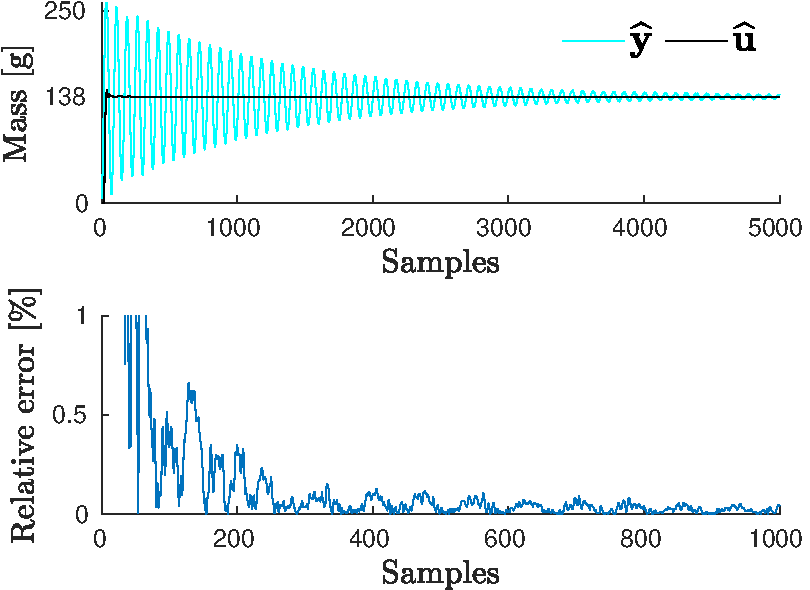
\includegraphics[width=1.0\columnwidth]{./ChapterExperimentalValidation/fig/Fig_1.pdf} 
\caption{ \label{fig:uh_sim} 
Above: example of a simulated response $\widehat{\mathbf{y}}$ and its step input estimation $\widehat{u}$ assuming measurement Gaussian noise with 50 dB of SNR. 
Below: the relative error $|\widehat{u} - u| / u$ is below 1\% after 100 samples. 
We take the estimate at 500 samples because there the relative error is smaller than 0.2\%.  }
\end{figure}

A sensor is a dynamic system, therefore, a fast measurement process must necessarily cope with the system transient response. In that respect we must distinguish between the transient response of the system under test, and the transient phase of the measurement process (i.e. before the process has settled on a final measurement outcome). Notice that the transient phase of the measurement process is considerably smaller than the settling time of the system under test, and this is a major advantage of the step input estimation method.

We are interested in the first element of $\widehat{\mathbf{x}}$, which is the input estimate $\widehat{u}$.
The measurement noise variance was selected to have a signal-to-noise ratio (SNR) in the interval [30 dB, 80 dB], according to
\begin{equation} \mathrm{SNR} = 20 \log_{10}{ \dfrac{ \sqrt{ \dfrac{1}{T} \int\limits_{0}^{T}{ y(\tau)^2  \mathrm{d} \tau } } }{ \sigma_{ \epsilon }} } \end{equation} 

The difference between the sample mean $\widehat{\mu}_u$ of the step input estimates and the true value $u$ is the empirical bias $b_\mathrm{e}$.
\begin{equation} {b}_\mathrm{e} = \frac{1}{N_{MC}} \sum_{i=1}^{N_{MC}}{ \widehat{u}_i - u } = \widehat{\mu}_u - u.  \end{equation}

The sample variance $\widehat{\sigma}_u^2$ of the step input estimates is used to obtain the standard error of the MC simulation $\sigma_\mathrm{e}$, which decreases with respect to the square root of the number of MC runs $N_{MC}$. 
\begin{equation}  \sigma_\mathrm{e} = \frac{\widehat{\sigma}_u}{\sqrt{N_{MC}}}, \ \mathrm{where} \ \ \widehat{\sigma}_u^2 = \frac{1}{N_{MC}-1} \sum_{i=1}^{N_{MC}}{ \left( \widehat{u}_i - \widehat{\mu}_u \right)^2 } . \end{equation}

In each of the $N_{MC}$ runs, we compute the predictions of the step input estimation bias and variance from measured data using Equations (\ref{eqn:biasST}) and (\ref{eqn:varST}). 
The step input bias and variance predictions from observed data $b_{\widetilde{\mathrm{p}}}$ and $v_{\widetilde{\mathrm{p}}}$, and the associated standard error $\sigma_{\widetilde{\mathrm{p}}}$, are obtained from
\begin{equation} \begin{aligned} & b_{\widetilde{\mathrm{p}}} = \frac{1}{N_{MC}} \sum_{i=1}^{N_{MC}}{ \mathbf{b}_{\widetilde{\mathrm{p}}}^i \left( \widehat{\mathbf{x}} \right) \big|_{\left[1\right]} }, \ v_{\widetilde{\mathrm{p}}} = \frac{1}{N_{MC}} \sum_{i=1}^{N_{MC}}{ \mathrm{\mathbf{C}}_{\widetilde{\mathrm{p}}}^i \left( \widehat{\mathbf{x}} \right) \big|_{\left[1,1\right]} },  \\ & \mathrm{and} \quad \sigma_{\widetilde{\mathrm{p}}} = \sqrt{   \frac{ \sum_{i=1}^{N_{MC}}{ \left( \mathbf{b}_{\widetilde{\mathrm{p}}}^i \left( \widehat{\mathbf{x}} \right) \big|_{\left[1\right]} - b_{\widetilde{\mathrm{p}}} \right)^2 } }{N_{MC}\left( N_{MC}-1 \right)}  } , \end{aligned} \end{equation}
where $\widetilde{\mathbf{b}}_{\mathrm{p}}^i \left( \widehat{\mathbf{x}} \right) \big|_{\left[1\right]}$ is the first element in the bias vector and $\widetilde{\mathbf{C}}_{\mathrm{p}}^i \left( \widehat{\mathbf{x}} \right) \big|_{\left[1,1\right]}$ is the first element in the covariance matrix obtained in the $i-\mathrm{th}$ approximations.
The predicted bias and variance from exact data are obtained with one evaluation of the expressions
(\ref{eqn:biasE}) and (\ref{eqn:varE})
\begin{equation} b_{\mathrm{p}} = \frac{1}{N_{MC}} \sum_{i=1}^{N_{MC}}{ \mathbf{b}_{\mathrm{p}} \left( \widehat{\mathbf{x}} \right) \big|_{\left[1\right]} }, \ \mathrm{and} \ v_{\mathrm{p}} = \frac{1}{N_{MC}} \sum_{i=1}^{N_{MC}}{ \mathrm{\mathbf{C}}_{\mathrm{p}} \left( \widehat{\mathbf{x}} \right) \big|_{\left[1,1\right]} } . \end{equation}
The uncertainty of the step input estimate is defined as the spread of the estimates that is given by the predicted variance $v_{\mathrm{p}}$.

Figure \ref{bias_sigma_sim_unstr_str_n2} shows the empirical bias, the bias predictions and the standard errors of the MC simulation.
It can be seen that the empirical bias $b_\mathrm{e}$ and the predicted bias $b_{\widetilde{\mathrm{p}}}$ are proportional to the perturbation noise variance while the standard errors $\sigma_\mathrm{e}$ and $\sigma_{\widetilde{\mathrm{p}}}$ are proportional to the perturbation noise standard deviation.
For SNR below 40 dB there is a difference of a small order of magnitude between the empirical bias $b_\mathrm{e}$ and the bias prediction $b_{\widetilde{\mathrm{p}}}$. 

The standard errors of the MC simulation $\sigma_\mathrm{e}$ and $\sigma_{\widetilde{\mathrm{p}}}$ are smaller than  $b_\mathrm{e}$ and $b_{\widetilde{\mathrm{p}}}$.
The estimates are spread near the sample mean and the uncertainty is smaller than the bias. 
Therefore, the empirical bias of the MC simulation is meaningful.

\begin{figure}[!htb]
\centering
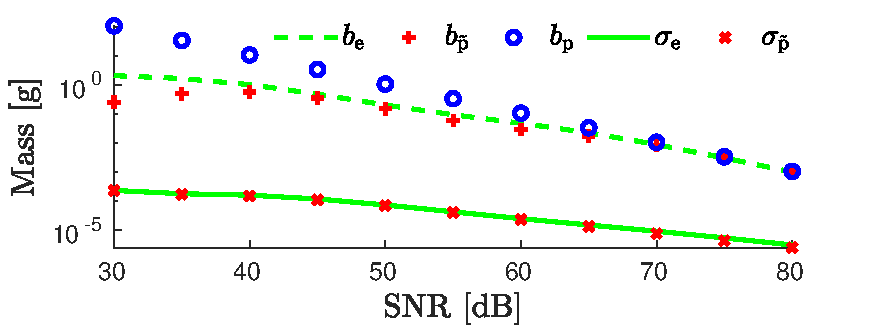
\includegraphics[width=1.0\columnwidth]{./ChapterExperimentalValidation/fig/Fig_2.pdf} 
\caption{ \label{bias_sigma_sim_unstr_str_n2} 
The results of the Monte Carlo simulation of the step input estimation method are the empirical bias $b_{\mathrm{e}}$, the predicted bias using exact data $b_{\mathrm{p}}$, the predicted bias using measured data $b_{\widetilde{\mathrm{p}}}$, the empirical standard error $\sigma_{\mathrm{e}}$, and the predicted standard error $\sigma_{\widetilde{\mathrm{p}}}$. The estimation biases are proportional to the perturbation variance and the estimation standard errors are proportional to the perturbation standard deviation. Since the standard errors are smaller than the biases, the MC simulation is meaningful.  }
\end{figure}

The mean squared error (MSE) of the step input estimate, defined as
\begin{equation} \mathrm{MSE} = b^2 + v,   \end{equation}
where $b$ and $v$ are the bias and the variance of the step input estimate, can be applied to the obtained empirical and predicted results and can be compared to the Cram\'er-Rao lower bound (CRB).
Figure \ref{fig:MSE_CRB} shows that $\mathrm{MSE}_\mathrm{e} = b_\mathrm{e}^2 + v_\mathrm{e}$ and $\mathrm{MSE}_{\widetilde{\mathrm{p}}}  = b_{\widetilde{\mathrm{p}}}^2 + v_{\widetilde{\mathrm{p}}}$ have the same proportionality with respect to the measurement noise variance as the bound for an unbiased estimator $\mathrm{CRB_{ub}}$.
For SNR above 35 dB, $\mathrm{MSE}_\mathrm{e}$ and $\mathrm{MSE}_{\widetilde{\mathrm{p}}}$ are equivalent, and below 35 dB the difference between them is of less than a factor of 10.

We obtained an approximation of the $\mathrm{CRB}_{\mathrm{b}}$ for our biased estimator using the partial derivative of the bias in expression (\ref{eqn:biasST}).
Figure \label{fig:MSE_CRB} shows that the bounds for the unbiased and biased estimators are almost equal because the partial derivatives of the bias are negligible w.r.t. 1 in Equation (\ref{eqn:CRB_EIV}).
By adding the square of the predicted bias to the biased estimator bound $\mathrm{CRB_{b}}$ we obtain an approximation of the minimum MSE that the biased estimator can achieve.
This minimum MSE is close to the CRBs for large SNR but the square of the bias causes an increase of the MSE around 35 dB.
The differences between the CRBs and $\mathrm{MSE}_\mathrm{e}$ and $\mathrm{MSE}_{\widetilde{\mathrm{p}}}$ are of one order of magnitude for large SNR and become small for SNR lower than 40 dB.
This difference is the cost of solving a structured EIV problem with a simple LS method.
%Therefore, for large measurement noise variance, the step input estimation method produces results that are comparable to maximum-likelihood estimation, since $\mathrm{MSE}_{\widetilde{\mathrm{p}}} \approx \mathrm{CRB_{b}} + b_{\widetilde{\mathrm{p}}}^2$.


\begin{figure}[!htb]
\centering
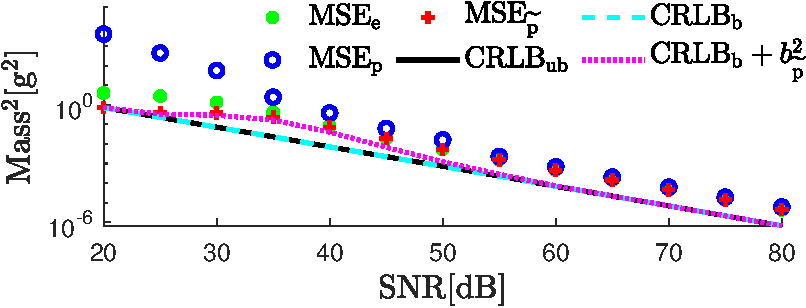
\includegraphics[width=1.0\columnwidth]{./ChapterExperimentalValidation/fig/Fig_3.pdf}
\caption{\label{fig:MSE_CRB} The observation instant is fixed at 500 samples.
The bias and the MSEs decrease for large SNR. 
The empirical $\mathrm{MSE_e}$ and the predicted $\mathrm{MSE}_{\widetilde{\mathrm{p}}}$ of the step input estimation are one order of magnitude larger than the Cram\'er-Rao lower bound.
Adding the CRB for a biased estimator with the predicted bias squared we have the minimum MSE, that grows in the interval [25 dB, 45 dB].
Below 35 dB the difference between $\mathrm{MSE}_{\widetilde{\mathrm{p}}}$ and the CRB is less than a factor of 10.}
\end{figure}

There are two features of the system step response that make the CRB small.
One is the measurement noise variance and the second is sample size.
The estimation from step response perturbed with small noise variance has lower uncertainty.
Also, using larger sample size to perform the estimation boils down to smaller estimation uncertainty.

In order to get more insight into the step input estimation method we conducted another simulation study. 
The step input estimation method assumes the order $n$ is given in (\ref{eqn:min_seiv}).
In this simulation, the step input estimation method processed the step response generated by a $5-th$ order system using different values of $n$ in the interval from 2 to 100.

The step response is perturbed with Gaussian white noise with SNR values in the interval [20 dB, 80 dB].
For each order $n$ and SNR value, 100 step input estimations are performed from independent noise realizations. 
Figure \ref{fig:msee_vs_n_sim} shows the average of the squared biases and the variances, and the MSEs of the input estimate using the first 500 samples.
It is evident that the estimation variance and MSE depend on the SNR.

Increasing the order $n$ is equivalent to adding more regressors in the regression problem.
It is well known that increasing the order $n$ causes a monotonic decrement of the estimation bias and increment of the variance.
This is the asymptotic behavior of the estimation statistical moments with respect to the number of regressors.
Nevertheless, the simulation results presented in Figure \ref{fig:msee_vs_n_sim} show that the variance first increases for small values of $n$, followed by a decrement and finally after $n \approx 40$ the variances exhibit a slow and steady increment. 
This apparent contradiction does not prove the invalidity of the estimation method since the results presented correspond to a finite sample size and the asymptotic results cannot be applied.
The theoretical explanation of the estimation statistics for finite sample sizes is out of the scope of this paper.

 
There is a bias-variance tradeoff and the MSEs exhibit local minima with respect to $n$.
The principal contribution to the MSE is the squared bias for the smaller values of $n$ and the variance for the larger values of $n$. 
However, the higher orders do not produce overfitting since the MSEs do not grow fast and remain close to the minimum values. 

The optimum value of $n$ is not necessarily equal to the order of the generating system and varies for each SNR.
According to the plots in Figure \ref{fig:msee_vs_n_sim}, there are orders that provide local minima of the step input estimation MSEs.
From the right hand side of Figure \ref{fig:msee_vs_n_sim}, the orders that give the first two MSE minima were identified and those values are listed in Table \ref{Tbl:orders}.
For each SNR, there is a first minimum at a low order and a second minimum at a high order.
For SNR of 30 and 40 dB, it is recommended to use the order that gives the first minimum since the MSE at the second minimum is less than one order of magnitude smaller than at the first minimum.
Depending on the requirements, the user can choose between the simplicity of an estimation with a low order or an estimation with higher computational complexity and a smaller MSE. 
In a calibration stage, during the setup of the estimation method, the user can search and set the order that enables the estimation method to provide a required MSE.



\begin{table}[!ht]
\caption{ Orders $n$ that provide local minima for the MSE of the step input estimate. It is recommended to use the order that gives the first minimum when there is a difference of small order of magnitude with respect to the MSE at the second minimum.} 
\label{Tbl:orders} 
\centering
\begin{tabular}{c|c c c c} 
\hline
SNR [dB] & 30 & 40 & 50 & 60 \\
\hline
order at first minimum & 11 & 7 & 4 & 3 \\ 
order at second minimum & 40 & 35 & 40 & 31 \\
\hline
\end{tabular}
\end{table}

\begin{figure}[!htbp]
\centering
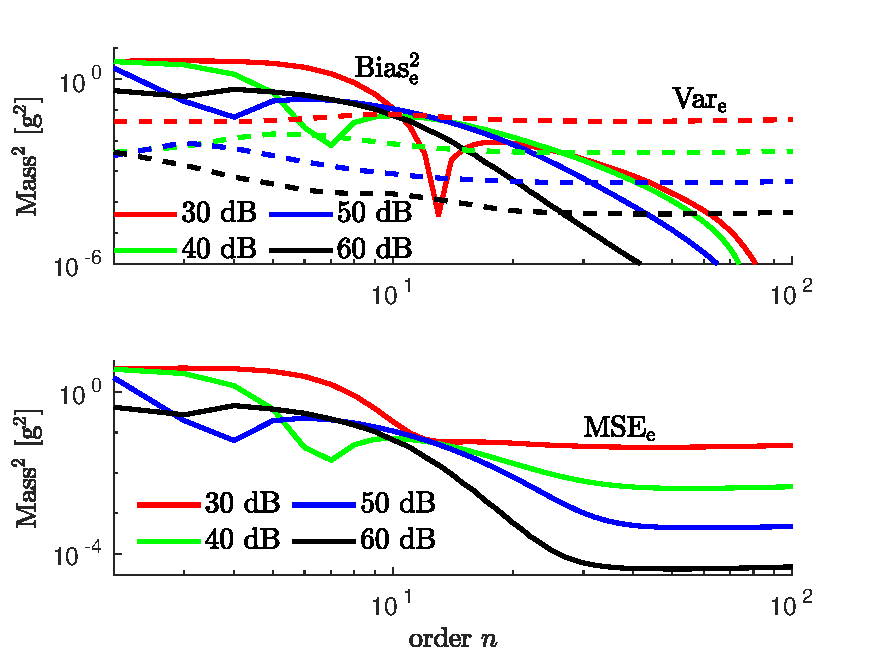
\includegraphics[width=\columnwidth]{./ChapterExperimentalValidation/fig/Fig_4.pdf} 
\caption{ \label{fig:msee_vs_n_sim} 
The simulated step responses of a $\mathrm{5-}th$ order system are processed by the step input estimation method using different orders $n$ and independent noise realizations. 
The perturbation of the step responses is Gaussian white noise with SNRs of 30, 40, 50, and 60 dB.
The square of the empirical bias (solid) and the empirical variance (dashed) are shown on the left hand side and the MSE is shown on the right hand side, for $n$ between 2 and 100.
These results suggest that, during the setup of the estimation method, we have to search the order that gives the minimum MSE without increasing unnecessarily the complexity of the estimation method.  }
\end{figure}


% \begin{figure}
% \centering
% \includegraphics[width=0.5\columnwidth]{./msee_vs_n_sim.pdf} 

%\end{figure}


\section{Practical implementation} 
An experimental setup was constructed to test the step input estimation method.
The implementation is a weighing system that uses a load cell Tedea Huntleigh 1004 \citep{tedea1004}.
The maximum rating of the load cell is 600 g.
A cylindrical aluminium object of 138.32 g of mass was used to excite the load cell.
This value was found by calibration using a balance KERN PCB 200-2 that has an uncertainty of 0.01 g.
The step input excitation was provided by a magnet that holds and releases a mass from above the load cell.
The magnet is located sufficiently far from the load cell to avoid magnetic interference in the sensor response.

\ctikzset{bipoles/resistor/height=0.075}
\ctikzset{bipoles/resistor/width=0.25}
\begin{figure}[!htb]
\centering
\begin{tikzpicture}[every node/.style={draw,outer sep=0pt,thick}]
\tikzstyle{spring}=[thick,decorate,decoration={zigzag,pre length=0.3cm,post length=0.3cm,segment length=6}]
\tikzstyle{damper}=[thick,decoration={markings,  
  mark connection node=dmp,
  mark=at position 0.5 with 
  {
    \node (dmp) [thick,inner sep=0pt,transform shape,rotate=-90,minimum width=15pt,minimum height=3pt,draw=none] {};
    \draw [thick] ($(dmp.north east)+(2pt,0)$) -- (dmp.south east) -- (dmp.south west) -- ($(dmp.north west)+(2pt,0)$);
    \draw [thick] ($(dmp.north)+(0,-5pt)$) -- ($(dmp.north)+(0,5pt)$);
  }
}, decorate]
\tikzstyle{ground}=[fill,pattern=north east lines,draw=none,minimum width=0.63cm,minimum height=0.3cm]

% load cell
\node (M1) [minimum width=1.6cm,minimum height=0.4cm, xshift=-3cm, yshift=-1cm] {};

\node (ground1) at (M1.east) [ground,yshift=0.0cm,rotate=90,xshift=0.0cm,anchor=north] {};
\draw (ground1.north east) -- (ground1.north west);

\node at (M1.north) [fill=none, xshift=-0.75cm, yshift=0.750cm] (2.0cm, 1.50cm) {\small Mass};
\draw (M1.north) [-latex,thick]  ++(-0.75cm,0.5cm) -- +(0cm,-0.5cm);
\draw (-3.3750cm,-0.935cm) arc(30:330:1.25mm);
\draw (-2.625cm,-1.05cm) arc(210:510:1.25mm);
\draw (M1.west) [thick]  ++(0.4cm, 0.0750cm) -- +(0.80cm,0.0cm);
\draw (M1.west) [thick]  ++(0.4cm,-0.0750cm) -- +(0.80cm,0.0cm);

\node at (M1.south) [align=center, draw=none,fill=none, xshift=0.0cm, yshift=-0.5cm] (2.0cm, 1.50cm) {\small load cell \\ \small Tedea 1004};

% amplifier
\draw (-1.6,-0.0) -- (-1.6,-2.0) -- (1.2,-1) -- cycle;
    \draw (-1.5,-1) to[R] (-1.1,-0.6) to[R] (-0.7,-1);
    \draw (-1.5,-1) to[R] (-1.1,-1.4) to[R] (-0.7,-1);
\draw [-latex,thick]  ++(1.2,-1) -- +(0.8,0);

\node (filter) [minimum width=0.50cm,minimum height=0.50cm, xshift=-0.0cm, yshift=-1cm] {};
\draw [thick]  ++(-0.275,-0.9) -- +(0.275,0.0);
\draw [thick]  ++(0,-0.9) -- +(0.25,-0.250);
\node at (M1.east) [draw=none, fill=none, xshift=4.0cm, yshift=0.25cm] (2.0cm, 1.50cm) {$\widetilde{y}$};
% wire
\draw plot [smooth] coordinates {(-2.3,-0.8) (-2.2,-0.5) (-1.7,-0.5) (-1.65,-0.9) (-1.6,-1)};

\node at (M1.south) [align=center, draw=none,fill=none, xshift=3.75cm, yshift=-0.750cm] (2.0cm, 1.50cm) {\small amplifier and filter};

\node (ADC) [align=center, minimum width=1.2cm,minimum height=0.9cm, xshift=2.6cm, yshift=-1cm] {\small ADC \\ \small 16 bits};

\end{tikzpicture}
\caption{Diagram of the load cell and the conditioning amplifier that provide the sensor response.} \label{lcm}
\end{figure}

A two-stage linear conditioning amplifier performs amplification and filtering of the load cell signal.
The first stage is a precision instrumentation amplifier INA114 that has high common mode rejection ratio.
The second stage is a third-order low-pass Butterworth filter with cut-off frequency of 100 Hz.
The low-pass filter prevents the aliasing noise in the measured transient response.
The signal obtained from the conditioning amplifier is considered to be the response of the sensor.
The sensor responses to step excitations were sampled with a frequency of $f_s=4$ kHz, and therefore the Nyquist frequency is 2 kHz.
The step responses were collected and stored as datasets for further analysis.
The number of samples collected for each step response is $N=20000$.
For practical purposes, we consider that the last 10000 samples correspond to the steady state response.
%The datasets are available in the following repository: %[[https://www.dropbox.com/sh/0dlam0rqqiynyiq/AAAq0H9rFxpkQON4zkmPXPXXa?dl=0][dropbox folder]]. 
\begin{figure}[!htb]
\centering
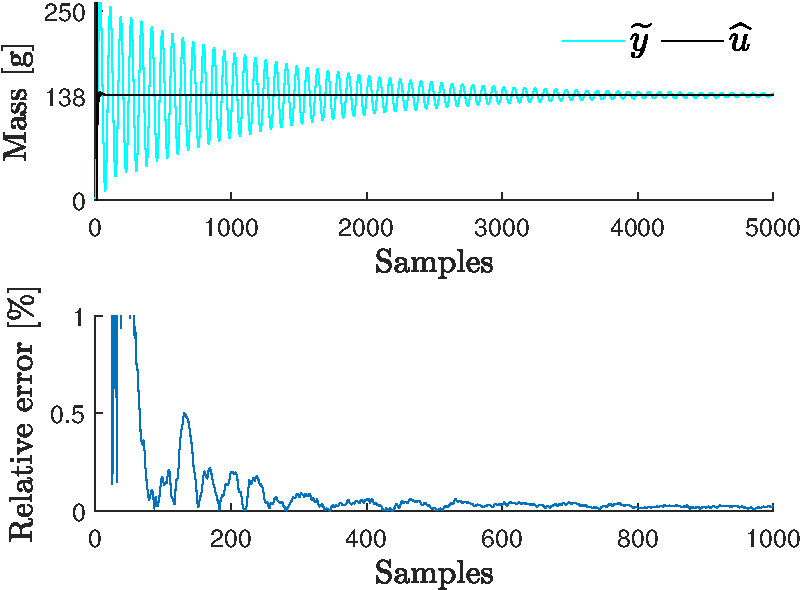
\includegraphics[width=1.0\columnwidth]{./ChapterExperimentalValidation/fig/Fig_6.pdf} 
\caption{ \label{fig:uh_exp} 
Above: a typical measured sensor transient response $\widetilde{y}$ takes more than 1.25 s (5000 samples, $f_s = 4$ kHz) to converge to the steady state response. 
Below: the relative error of the input estimate $\widehat{u}$ is smaller than 0.2\% from 300 samples.
We consider that at $500$ samples the relative error of the estimate $\widehat{u}$ is small enough to consider that $\widehat{u}$ is close to its expected value $u$.  }
\end{figure}

The step input estimation method processed 100 measured sensor step responses, assuming the sensor is of $\mathrm{7-}th$ order.
Figure \ref{fig:uh_exp} shows a typical measured transient response $\widetilde{y}$ and an example of the estimated input $\widehat{u}$.

The empirical bias $b_{\mathrm{e}}$ is the difference between the average of the 100 estimates $\widehat{u}$ and the mass calibration value $u = 138.32$ g, at each instant of time, and the standard error $\sigma_\mathrm{e}$ is the standard deviation of the mean estimate of the responses processed, i.e.,
\begin{equation} \begin{aligned} \widehat{\mu}_{e} &= \frac{1}{100} \sum_{i=1}^{100}{ \widehat{u}_{i} }, \quad {b}_{\mathrm{e}} = \widehat{\mu}_{e} - u, \quad \mathrm{and} \\  \sigma_{\mathrm{e}} &= \frac{\widehat{\sigma}}{\sqrt{100}}, \quad \mathrm{where} \ \widehat{\sigma}^2 = \frac{1}{99} \sum_{i=1}^{100}{ \left( \widehat{u}_i - \widehat{\mu}_{e} \right)^2 } . \end{aligned} \end{equation}


The bias $\widetilde{b}_{\mathrm{p}}$ and variance $\widetilde{v}_{\mathrm{p}}$ predictions from the measured data were obtained by processing off-line the 100 measured sensor transient step responses with expressions (\ref{eqn:biasST}) and (\ref{eqn:varST}).
These expressions require the measurement noise variance $\sigma_\epsilon^2$ to obtain the bias and variance prediction.
One way to estimate the measurement noise variance is computing the variance of each sensor steady state response, see Figure \ref{fig:y_ss}.
Later in this section we will explore another way to estimate the measurement noise variance.
Computing the noise variance from the steady state response we observed that the SNR of the measured step responses is 55 dB in average.

\begin{figure}[!htb]
\centering
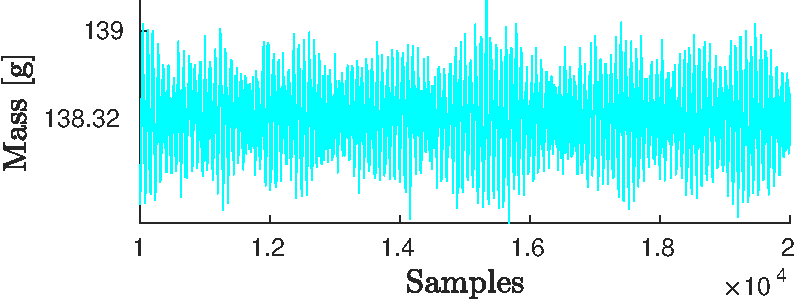
\includegraphics[width=1.0\columnwidth]{./ChapterExperimentalValidation/fig/Fig_7.pdf}
\caption{ \label{fig:y_ss} 
From the sensor steady-state response an estimation of the measurement noise variance is obtained.}
\end{figure}

Figure \ref{fig:b_sigma_exp_str} shows the empirical bias $b_{\mathrm{e}}$ and the standard error $\sigma_{\mathrm{e}}$ that result after processing the first $T=500$ samples of the 100 measured step responses $\widetilde{\mathbf{y}}$.
The standard error is smaller than the bias.
As it was observed in the MC simulation, this is the uncertainty of the estimation method.
The oscillations observed in the bias are mainly due to the transient response and not to the measurement noise.
The measurement noise effects are partially removed since we averaged the 100 transient responses, 
which is a small number compared with the $N_{MC}$ runs averaged in the simulation section. 

It is expected that the empirical bias is large when a small number of samples is processed. 
The data-driven input estimation method is recursive and it is implemented in real-time.
The estimation errors decrease as more data is processed.

\begin{figure}[!htb]
\centering
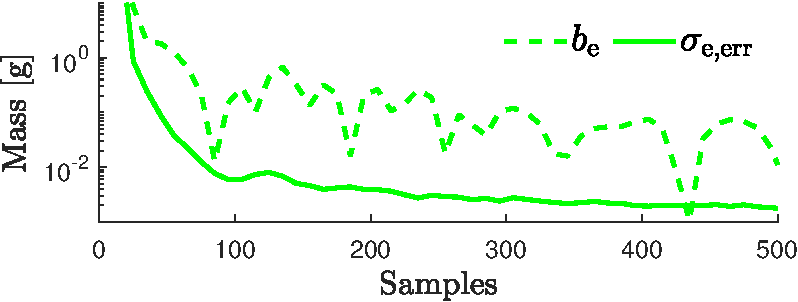
\includegraphics[width=1.0\columnwidth]{./ChapterExperimentalValidation/fig/Fig_8.pdf} 
\caption{ \label{fig:b_sigma_exp_str} 
The results of estimating the step input level after processing 100 measured step responses are the empirical bias $b_{\mathrm{e}}$ and the empirical standard error $\sigma_{\mathrm{e}}$. 
The estimation bias and the estimation standard error decrease as more samples are processed. 
The estimation bias is affected by the transient effects of the sensor response.  
The values of $b_{\mathrm{e}}$ and $\sigma_{\mathrm{e}}$ provide the estimate accuracy and uncertainty for a given sample size.
}
\end{figure}

The measurement noise is not white since there is evidence of frequency components in the sensor steady state response that are observed as oscillations in Fig \ref{fig:y_ss}.
To get insight into the properties of the measured sensor response $\widetilde{\mathbf{y}}$, a $\mathrm{7-}th$ order model was identified from input-output data assuming that the input is a step of level $u$.
A response $\widehat{\mathbf{y}}$ was simulated from the identified model and the residual $\mathbf{r} = \widetilde{\mathbf{y}} - \widehat{\mathbf{y}}$ was obtained. 
We can observe these signals in the frequency domain using the discrete Fourier transform, that for the signal $\widetilde{\mathbf{y}}$ is defined as 
\begin{equation} \widetilde{Y}(f) = \dfrac{1}{\sqrt{N}} \sum_{k=0}^{N-1} \widetilde{y} \left( k \right) e^{-j2\pi k f / N} \label{eqn:FFT} \end{equation}
where $f = 1, \ldots, N/2$ are the frequency lines and $N$ is the total number of samples.
The power spectrum of the signal $\widetilde{\mathbf{y}}$ is given in decibels by $\widetilde{\mathbf{Y}}_\mathrm{dB} = 20 \log_{10}{ |\widetilde{\mathbf{Y}}| } $.
Figure \ref{fig:YYhR_n7} shows the corresponding power spectra of the sensor response $\widetilde{\mathbf{Y}}_\mathrm{dB}$, the simulated response $\widehat{\mathbf{Y}}_\mathrm{dB}$, and the residual $\mathbf{R}_\mathrm{dB}$. 
There are frequency components near the main resonance peak in the magnitude spectrum of the residual.
The presence of frequency components near the main resonance peak is commonly found in mechanical devices.
The vibrations captured from the environment explain the accumulation of energy near the main resonance modes.

\begin{figure}[!htb]
\centering
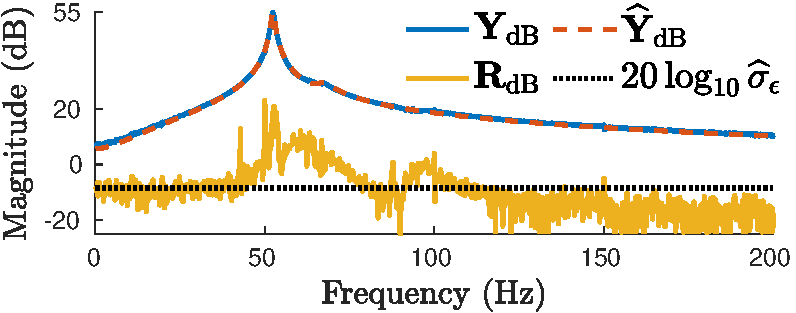
\includegraphics[width=1.0\columnwidth]{./ChapterExperimentalValidation/fig/Fig_9.pdf}
\caption{ \label{fig:YYhR_n7} 
The power spectra of a measured response $\widetilde{\mathbf{Y}}_\mathrm{dB}$, a simulated response $\widehat{\mathbf{Y}}_\mathrm{dB}$, and the residual $\mathbf{R}_\mathrm{dB}$ is not flat and then the measurement noise is not white. 
The average of the residual power spectrum provides a conservative estimate of the measurement noise variance $\widehat{\sigma}_\epsilon^2$, represented with the dotted line.}
\end{figure}

Even when the residual $\mathbf{r}$ is not white, it provides an alternative way to estimate the measurement noise variance. 
The average of the residual power spectrum approximates the measurement noise variance as follows
\begin{equation} \widehat{\sigma}_\epsilon^2 \approx \dfrac{2}{N} \sum_{f = 1}^{N/2} \left| R \left( f \right) \right|^2 . \label{eqn:P_R} \end{equation}
The dotted line in Figure \ref{fig:YYhR_n7} indicates the $10 \log_{10} \left( \widehat{\sigma}_\epsilon^2 \right)$ level of the measurement noise variance estimated from the residual.
This level is higher than the mean value of the residual power spectrum $\mathbf{R}_\mathrm{dB}$ in the frequencies above 120 Hz.

Using the residual power spectra that correspond to the measured step responses, we obtained the measurement noise variance and the SNR for each experiment.
Figure \ref{fig:meas_SNR} shows the estimated SNRs from the residual power spectra. 
The SNR mean value is 50 dB.
Therefore, we assume that the SNR of the measured transient responses is 50 dB instead of 55 dB, as it was estimated from the steady state response.

\begin{figure}[!htb]
\centering
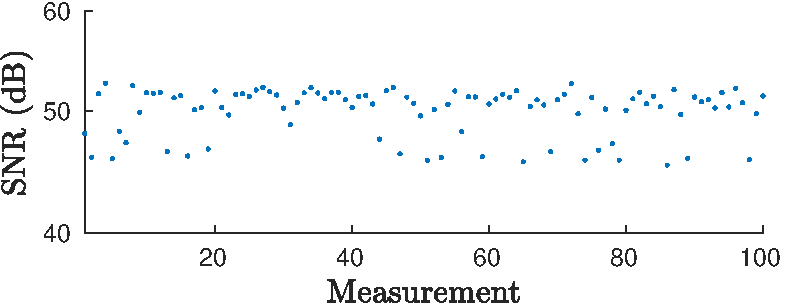
\includegraphics[width=1.0\columnwidth]{./ChapterExperimentalValidation/fig/Fig_10.pdf}
\caption{ \label{fig:meas_SNR} 
The mean value of the signal-to-noise ratios estimated from the residual power spectra is 50 dB.
We consider that this is the estimated SNR of the measured step responses.}
\end{figure}

The 5 dB difference provides a conservative bound since the bias and variance computed from 50 dB of SNR are higher than those obtained using the variance estimation from the steady-state response. 
Figure \ref{fig:b_sigma_exp_str2} shows a comparison of the results obtained with both measurement noise variance estimations after processing the first $T=500$ samples of the step response $\widetilde{\mathbf{y}}$.
Using expression (\ref{eqn:biasST}), the bias prediction  $b_{\widetilde{\mathrm{p}}2}$ obtained using an SNR of 50 dB approximates more closely the empirical bias than $b_{\widetilde{\mathrm{p}}1}$ obtained using an SNR of 55dB.
In accordance, the standard error of the bias predictions $\sigma_{\widetilde{\mathrm{p}}2}$ is larger than $\sigma_{\widetilde{\mathrm{p}}1}$ and is a conservative measure of the input estimation uncertainty.
In conclusion, using the noise variance estimated from the residual prevents underestimating the step input estimation uncertainty.


\begin{figure}[!htb]
\centering
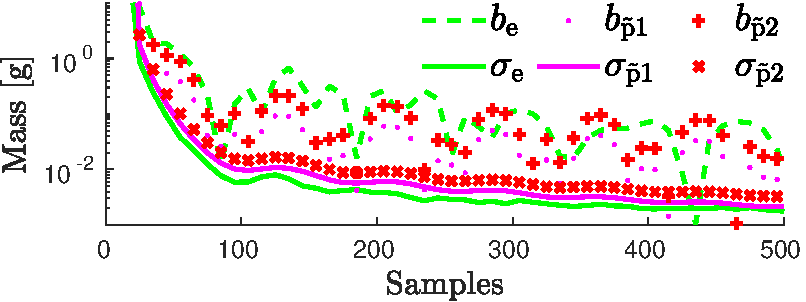
\includegraphics[width=1.0\columnwidth]{./ChapterExperimentalValidation/fig/Fig_11.pdf} 
\caption{ \label{fig:b_sigma_exp_str2} 
Comparative view of the bias prediction using two different noise variance estimations. 
Estimating the variance from the step response residual gives a bias prediction $b_{\widetilde{\mathrm{p}}2}$ and a standard error $\sigma_{\widetilde{\mathrm{p}}2}$ that are slightly higher than using the noise variance estimated from the steady state response $\sigma_{\widetilde{\mathrm{p}}1}$ and $\sigma_{\widetilde{\mathrm{p}}1}$. 
The bias prediction $b_{\widetilde{\mathrm{p}}2}$ approximates better the empirical bias. 
The standard error $\sigma_{\widetilde{\mathrm{p}}2}$ provides a conservative value of the input estimation uncertainty. }
\end{figure}


We investigated another aspect of the step input estimation method performance when processing measured step responses.
The step input estimation method requires an assumption of the generating system order in the formulation of the estimation problem (\ref{eqn:min_seiv}).
The estimation method performance is assessed under different assumptions of the values of $n$ in the interval from 2 to 10. 
For each value of $n$, 100 step input estimations are computed from measured transient responses and the empirical MSEs are compared.
Figure \ref{fig:msee_vs_n_exp} shows that, similar to the observations made in the simulation study, the MSEs have two local minima at $n=7$ and $n=48$.
It is recommended to use $n = 7$ in the estimation method to provide a small estimation MSE without the higher computational complexity that $n=48$ implies.


\begin{figure}[!htbp]
\centering
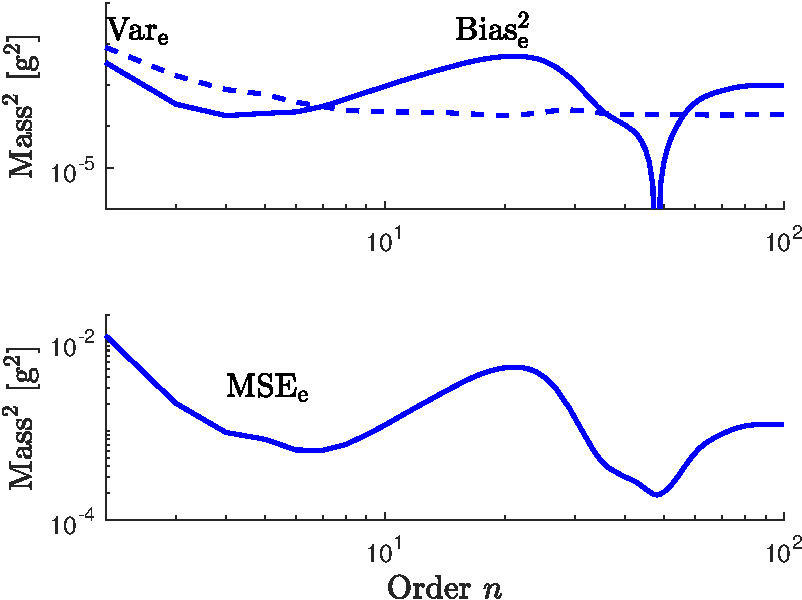
\includegraphics[width=1.0\columnwidth]{./ChapterExperimentalValidation/fig/Fig_12.pdf} 
\caption{ \label{fig:msee_vs_n_exp} 
The hundred measured sensor step responses are processed by the step input estimation method for different values of the order $n$. 
The empirical squared bias (solid) and the empirical variance (dashed) are shown on the left and the empirical MSE on the right.
The MSE has a local minimum at $n=7$ and another at $n=48$.
It is recommended to use the estimation method with $n=7$ because at $n=48$ the decrement of the MSE is not significant.  }
\end{figure}

\section{Conclusions}

In this paper we investigated the statistical properties of a data-driven step input estimation method in a real-life application.
The step input estimation method is a structured and correlated errors-in-variables problem that is solved with recursive least squares.
A statistical analysis was conducted using the ordinary least squares condensed notation. 
This statistical analysis of the input estimate provides expressions that approximate the estimation bias and variance assuming that the measurement noise is Gaussian white noise. 
The variance approximation is useful to assess the uncertainty of the input estimate.
In simulation we observed that the mean squared error of the input estimate is close to the theoretical minimum that uses the Cram\'er-Rao lower bound for biased estimators.
Since the data-driven step input estimation method is not statistically efficient, there is room for improvement. This is a topic for future research.
In the practical experiments, the measurement noise is not white.
The noise variance obtained from the sensor steady state response underestimates the measurement noise variance, that was observed 5 dB larger in the power spectrum due to nonlinearities of the sensor.
Considering this difference in the measurement noise variance, we introduced a conservative bound of the measurement noise variance so that the first and second moments of the input estimate are more accurately predicted.
Using the variance approximation, we can assess the uncertainty of the input estimate with respect to the number of samples processed by the data-driven step input estimation method.
The step input estimation method is useful in practical applications where the whiteness assumption of the measurement noise is not fulfilled. 


\newpage

